\documentclass{article}

\usepackage{graphicx}
\usepackage{rotating}
\usepackage{amsmath}
\usepackage{fancyhdr}
\usepackage{listings}
\usepackage{xcolor}
\usepackage{color}
\usepackage{textcomp}
\usepackage{float}
\usepackage{multirow}
\usepackage[sorting=none]{biblatex}
\usepackage[margin=1in]{geometry}
\usepackage[font={small,it}]{caption}
\usepackage{placeins}
\usepackage{xepersian}

%\DeclareMathOperator*{\btie}{\bowtie}
\addbibresource{bibliography.bib}
\settextfont[Scale=1.2]{B-NAZANIN.TTF}
\setlatintextfont[Scale=1]{Times New Roman}
\renewcommand{\baselinestretch}{1.5}
\pagestyle{fancy}
\fancyhf{}
\rhead{تکلیف دوم درس مبانی بینایی کامپیوتر}
\lhead{\thepage}
\rfoot{علیرضا ابره فروش}
\lfoot{9816603}
\renewcommand{\headrulewidth}{1pt}
\renewcommand{\footrulewidth}{1pt}
%%%%%%%%%%
\lstset
{
    language=[latex]tex,
    basicstyle=\ttfamily,
    commentstyle=\color{black},
    columns=fullflexible,
    keepspaces=true,
    upquote=true,
    showstringspaces=false,
    morestring=[s]\\\%,
    stringstyle=\color{black},
}
%%%%%%%%%%
%beginMatlab
\definecolor{mygreen}{RGB}{28,172,0} % color values Red, Green, Blue
\definecolor{mylilas}{RGB}{170,55,241}
%endMatlab
\begin{document}
%beginMatlab
\lstset{language=Matlab,%
    %basicstyle=\color{red},
    breaklines=true,%
    morekeywords={matlab2tikz},
    keywordstyle=\color{blue},%
    morekeywords=[2]{1}, keywordstyle=[2]{\color{black}},
    identifierstyle=\color{black},%
    stringstyle=\color{mylilas},
    commentstyle=\color{mygreen},%
    showstringspaces=false,%without this there will be a symbol in the places where there is a space
    numbers=left,%
    numberstyle={\tiny \color{black}},% size of the numbers
    numbersep=9pt, % this defines how far the numbers are from the text
    emph=[1]{for,end,break},emphstyle=[1]\color{red}, %some words to emphasise
    %emph=[2]{word1,word2}, emphstyle=[2]{style},    
}
%endMatlab
\begin{titlepage}
\begin{center}

\includegraphics[width=0.4\textwidth]{figures/IUT Logo.png}\\
        
\LARGE
\textbf{دانشگاه صنعتی اصفهان}\\
\textbf{دانشکده مهندسی برق و کامپیوتر}\\
        
\vfill
        
\huge
\textbf{عنوان: تکلیف چهارم درس ریزپردازنده}\\
        
\vfill
        
\LARGE
\textbf{نام و نام خانوادگی: علیرضا ابره فروش}\\
\textbf{شماره دانشجویی: 9816603}\\
\textbf{نیم\,سال تحصیلی: پاییز 1400}\\
\textbf{مدرّس: دکتر عارف کریمی افشار}\\
\end{center}
\end{titlepage}


%\tableofcontents
\newpage


\section{}%1
ابتدا متغیرهای زیر را تعریف می‌کنیم.
\newline
$H$ و $W$: ابعاد تصویر
\newline
$I$: تصویر اصلی
\newline
$J$: تصویر مورد بررسی
\newline
$MAX_{I}$: بزرگ‌ترین سطح روشنایی محتمل در تصویر (مقدار پیش‌فرض 255)
\newline
$MIN_{I}$: کوچک‌ترین سطح روشنایی محتمل در تصویر (مقدار پیش‌فرض 0)

\subsection{\lr{MAE}}
\subsubsection{حداکثر}
حالتی را تصور می‌کنیم که اختلاف سطح روشنایی هر دو پیکسل متناظر در تصویر حداکثر باشد (تصویر تمام سیاه و تمام سفید). بنابراین به ازای هر $i$ و $j$ دامنه، $I(i, j)$ برابر $MAX_{I}$ و $J(i, j)$ برابر $MIN_{J}$ یا بالعکس. پس داریم:
\newline
\begin{latin}
$
\max(\frac{1}{H.W}\sum_{i=1}^{H}\sum_{j=1}^{W}\left| I(i, j) - J(i, j) \right|)=\frac{1}{H.W}\times H.W\times \left| MAX_{I} - MIN_{J} \right|=\left| MAX_{I} - MIN_{J} \right|
$
\end{latin}
که در حالت پیش‌فرض این مقدار برابر 255 است.
\subsubsection{حداقل}
حالتی را تصور می‌کنیم که اختلاف سطح روشنایی هر دو پیکسل متناظر در تصویر حداقل باشد (تصاویر برابر باشند). بنابراین به ازای هر $i$ و $j$ دامنه، $I(i, j)$ برابر $J(i, j)$ است. پس داریم:
\newline
\begin{latin}
$
\min(\frac{1}{H.W}\sum_{i=1}^{H}\sum_{j=1}^{W}\left| I(i, j) - J(i, j) \right|)=\frac{1}{H.W}\times H.W\times \left| I(i, j) - I(i, j) \right|=0
$
\end{latin}


\subsection{\lr{MSE}}
\subsubsection{حداکثر}
مشابه قسمت قبل، حالتی را تصور می‌کنیم که اختلاف سطح روشنایی هر دو پیکسل متناظر در تصویر حداکثر باشد (تصویر تمام سیاه و تمام سفید). بنابراین به ازای هر $i$ و $j$ دامنه، $I(i, j)$ برابر $MAX_{I}$ و $J(i, j)$ برابر $MIN_{J}$ یا بالعکس. پس داریم:
\newline
\begin{latin}
$
\max(\frac{1}{H.W}\sum_{i=1}^{H}\sum_{j=1}^{W} (I(i, j) - J(i, j))^{2})=\frac{1}{H.W}\times H.W\times (MAX_{I} - MIN_{J})^{2}=(MAX_{I} - MIN_{J})^{2}
$
\end{latin}
که در حالت پیش‌فرض این مقدار برابر 65025 است.
\subsubsection{حداقل}
مشابه قسمت قبل، حالتی را تصور می‌کنیم که اختلاف سطح روشنایی هر دو پیکسل متناظر در تصویر حداقل باشد (تصاویر برابر باشند). بنابراین به ازای هر $i$ و $j$ دامنه، $I(i, j)$ برابر $J(i, j)$ است. پس داریم:
\newline
\begin{latin}
$
\min(\frac{1}{H.W}\sum_{i=1}^{H}\sum_{j=1}^{W} (I(i, j) - J(i, j))^{2})=\frac{1}{H.W}\times H.W\times (I(i, j) - I(i, j))^{2}=0
$
\end{latin}


\subsection{\lr{PSNR}}
برای بیشینه (کمینه) کردن تابعِ 
$
10\log_{10}(\frac{MAX_{I}^{2}}{MSE})
$
کافیست تابعِ
$
\frac{MAX_{I}^{2}}{MSE}
$
بیشینه (کمینه) کنیم.
\subsubsection{حداکثر}
با فرض ناصفر بودن مقدار $MAX_{I}$ داریم:
\newline
\begin{latin}
$
\max(10\log_{10}(\frac{MAX_{I}^{2}}{MSE}))=\lim_{MSE \to 0 } (10\log_{10}(\frac{MAX_{I}^{2}}{MSE}))=\infty
$
\end{latin}
پس به ازای دو تصویر با \lr{MSE}ِ نزدیک به صفر (دو تصویر تقریبا برابر)، مقدار \lr{PSNR} به بی‌نهایت میل می‌کند.
\subsubsection{حداقل}
اگر $I$ تصویر تمام سیاه ($MAX_{I}$ ناچیز باشد)، و $J$ تصویر غیر تمام سیاه باشد، آنگاه چون
$MAX_{I}$
تقریبا صفر است داریم:
\newline
\begin{latin}
$
\min(10\log_{10}(\frac{MAX_{I}^{2}}{MSE}))=\lim_{MAX_{I} \to 0 } (10\log_{10}(\frac{MAX_{I}^{2}}{MSE}))=-\infty
$
\end{latin}







\section{}%2
سطح روشنایی هر پیکسل در تصویر خاکستری‌گونه از $MIN_{I}$ (پیش‌فرض 0) تا $MAX_{I}$ (پیش‌فرض 255) متغیر است. بدترین \lr{MSE} که در واقع بزرگ‌ترین \lr{MSE} است زمانی رخ می‌دهد که اختلاف سطح روشنایی هر دو پیکسل متناظر در تصاویر ماکسیمم باشد. در نتیجه برای ساخت چنین تصویری فاصله‌ی سطح روشنایی هر پیکسل در تصویر اولیه را از مقادیر $MIN_{I}$ و $MAX_{I}$ به دست می‌آوریم (قدر مطلق تفاضل). در صورتی که سطح روشنایی به $MIN_{I}$ (سیاه) نزدیک‌تر بود، مقدار $MAX_{I}$ (سفید) و در صورتی که به $MAX_{I}$ (سفید) نزدیک‌تر بود، مقدار $MIN_{I}$ (سیاه) را در پیکسل متناظر قرار می‌دهیم. در این حالت چون قدر مطلق تفاضل‌ها به ازای همه پیکسل‌های تصویر ماکسیمم هستند پس تضمین می‌شود که ماکسیمم \lr{MSE}(بدترین \lr{MSE}) را نسبت به تصویر ورودی داریم.





\section{}%3
\subsection{الف}
\subsubsection{\lr{Function}}
\begin{latin}
\lstinputlisting{sources/toBlackWhite.m}
\end{latin}
\subsubsection{\lr{Driver code}}
\begin{latin}
\lstinputlisting{sources/p3a.m}
\end{latin}

\subsection{ب}
\subsubsection{\lr{Function}}
\begin{latin}
\lstinputlisting{sources/floydSteinberg.m}
\end{latin}
\subsubsection{\lr{Driver code}}
\begin{latin}
\lstinputlisting{sources/p3b.m}
\end{latin}

\subsection{ج}
\begin{latin}
\lstinputlisting{sources/p3c.m}
\end{latin}
با مقایسه‌ی \lr{PSNR} در دو تصویر تولید شده در قسمت‌های قبل درمی‌یابیم که بهتر بودن \lr{PSNR}ِ یک تصویر نسبت به تصویر دیگر الزاما به معنی بهتر بودن کیفیت بصری آن تصویر نیست. همانطور که می‌بینیم، تصویر تولید شده توسط الگوریتم \lr{Floyd-Steinberg} با وجود داشتن \lr{PSNR}ِ پایین‌تر نسبت به تصویر تولید شده توسط الگوریتم حریصانه (تابع \lr{toBlackWhite}) جزئیات تصویر را بهتر مشخص می‌کند و کیفیت بصری بهتری دارد. پس نتیجه می‌گیریم که \lr{PSNR} در همه جا معیار دقیقی برای مقایسه‌ی کیفیت تصاویر نیست.
\begin{figure}[H]
    \centering
    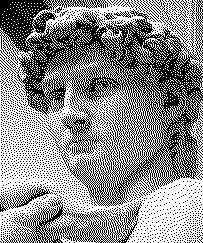
\includegraphics[width=0.25\textwidth]{figures/3c1.jpg}
    \caption
	{
خروجی الگوریتم \lr{Floyd-Steinberg}
	}
    \label{fig:fig1}
\end{figure}
\begin{figure}[H]
    \centering
    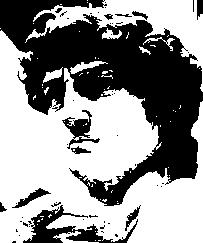
\includegraphics[width=0.25\textwidth]{figures/3c2.jpg}
    \caption
	{
خروجی الگوریتم حریصانه
	}
    \label{fig:fig1}
\end{figure}


\section{}%4
\subsection{\lr{Function}}
\begin{latin}
\lstinputlisting{sources/My_Imresize_BL.m}
\end{latin}
\subsection{\lr{Driver code}}
\begin{latin}
\lstinputlisting{sources/p4.m}
\end{latin}
\subsection{نمونه خروجی}
\begin{figure}[H]
    \centering
    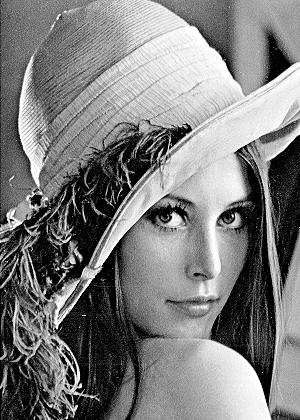
\includegraphics[width=0.25\textwidth]{figures/4a.jpg}
    \caption
	{
تصویر اصلی
	}
    \label{fig:fig1}
\end{figure}
\begin{figure}[H]
    \centering
    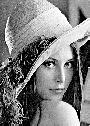
\includegraphics[width=0.25\textwidth]{figures/4b.jpg}
    \caption
	{
تصویر با ابعاد 30 درصد ابعاد تصویر اصلی
	}
    \label{fig:fig1}
\end{figure}


\section{}%5
پیکسل‌های تصویر را به طور یک در میان به شکل زیر می‌چینیم:
\begin{figure}[H]
    \centering
    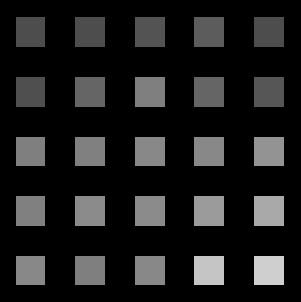
\includegraphics[width=0.25\textwidth]{figures/5a.jpg}
    \caption
	{}
    \label{fig:fig1}
\end{figure}
سطح روشنایی پیکسل‌های قرار گرفته در سطر زوج و ستون زوج را برابر با میانگین پیکسل‌های مجاور (4 پیکسل مشخص شده در شکل زیر در صورت وجود) قرار می‌دهیم. سطح روشنایی پیکسل‌های مرزی که دارای 2 همسایه‌ی مورب و 1 همسایه‌ی مورب هستند را هم به همین صورت مقداردهی می‌کنیم.

\begin{figure}[H]
    \centering
    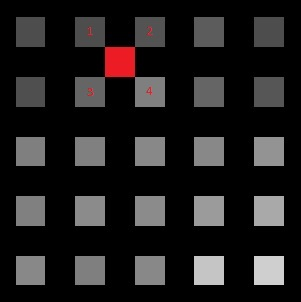
\includegraphics[width=1.0\textwidth]{figures/5b.jpg}
    \caption
	{}
    \label{fig:fig1}
\end{figure}
پیکسل‌ها تصویر به شکل زیر در می‌آیند:
\begin{figure}[H]
    \centering
    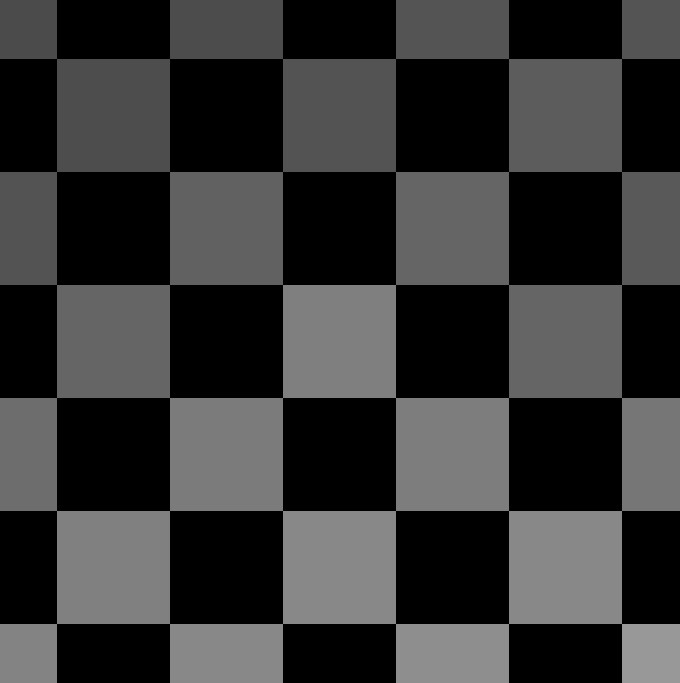
\includegraphics[width=0.25\textwidth]{figures/5c.jpg}
    \caption
	{}
    \label{fig:fig1}
\end{figure}
در گام بعد، سطح روشنایی پیکسل‌های باقی‌مانده را برابر میانگین پیکسل‌های مجاور (بالا، پایین، چپ و راست) قرار می‌دهیم. سطح روشنایی پیکسل‌های مرزی هم به طریق مشابه تعیین می‌شوند. این الگوریتم در تابعِ \lr{doubleDimensions} به شکل زیر پیاده‌سازی شده است.
\subsection{\lr{Function}}
\begin{latin}
\lstinputlisting{sources/doubleDimensions.m}
\end{latin}
\subsection{\lr{Driver Code}}
\begin{latin}
\lstinputlisting{sources/p5.m}
\end{latin}
جدول مقادیرِ \lr{PSNR} به شکل زیر می‌باشد.

%table
% Please add the following required packages to your document preamble:
% \usepackage{multirow}
\begin{table}[H]
\begin{tabular}{|ccccc|c|}
\hline
\multicolumn{5}{|c|}{\textbf{مقدار \lr{PSNR} به ازای \lr{Resizing\_Factor} برابر با 2}}                                                                                                                                                        & \multirow{2}{*}{\textbf{نام تصویر}} \\ \cline{1-5}
\multicolumn{1}{|c|}{\textbf{زمان اجرا بر حسب ثانیه}} & \multicolumn{1}{c|}{\textbf{روش پیشنهادی شما}} & \multicolumn{1}{c|}{\textbf{روش \lr{Bicubic}}} & \multicolumn{1}{c|}{\textbf{روش \lr{Bilinear}}} & \textbf{روش \lr{Nearest Neighbor}} &                                     \\ \hline
\multicolumn{1}{|c|}{\textbf{\lr{0.899658}}}          & \multicolumn{1}{c|}{\textbf{\lr{28.8864}}}     & \multicolumn{1}{c|}{\textbf{\lr{26.9296}}}     & \multicolumn{1}{c|}{\textbf{\lr{27.1040}}}      & \textbf{\lr{25.5147}}              & \textbf{\lr{Boat}}                  \\ \hline
\multicolumn{1}{|c|}{\textbf{\lr{0.941563}}}          & \multicolumn{1}{c|}{\textbf{\lr{32.1106}}}     & \multicolumn{1}{c|}{\textbf{\lr{29.7193}}}     & \multicolumn{1}{c|}{\textbf{\lr{29.9490}}}      & \textbf{\lr{28.1116}}              & \textbf{\lr{Peppers}}               \\ \hline
\multicolumn{1}{|c|}{\textbf{\lr{0.913748}}}          & \multicolumn{1}{c|}{\textbf{\lr{34.6318}}}     & \multicolumn{1}{c|}{\textbf{\lr{30.4896}}}     & \multicolumn{1}{c|}{\textbf{\lr{30.3392}}}      & \textbf{\lr{28.0316}}              & \textbf{\lr{Cameraman}}             \\ \hline
\multicolumn{1}{|c|}{\textbf{\lr{0.228155}}}          & \multicolumn{1}{c|}{\textbf{\lr{31.5815}}}     & \multicolumn{1}{c|}{\textbf{\lr{29.2722}}}     & \multicolumn{1}{c|}{\textbf{\lr{29.3679}}}      & \textbf{\lr{27.5452}}              & \textbf{\lr{House}}                 \\ \hline
\multicolumn{1}{|c|}{\textbf{}}                       & \multicolumn{1}{c|}{\textbf{\lr{31.802575}}}   & \multicolumn{1}{c|}{\textbf{\lr{29.102675}}}   & \multicolumn{1}{c|}{\textbf{\lr{29.190475}}}    & \textbf{\lr{27.30075}}             & \textbf{متوسط \lr{PSNR}}            \\ \hline
\end{tabular}
\end{table}
%table



\section{}%6
\subsection{الف}
\subsubsection{\lr{Function}}
\begin{latin}
\lstinputlisting{sources/myHist.m}
\end{latin}
\subsubsection{\lr{Driver code}}
\begin{latin}
\lstinputlisting{sources/p6a.m}
\end{latin}
\begin{figure}[H]
    \centering
    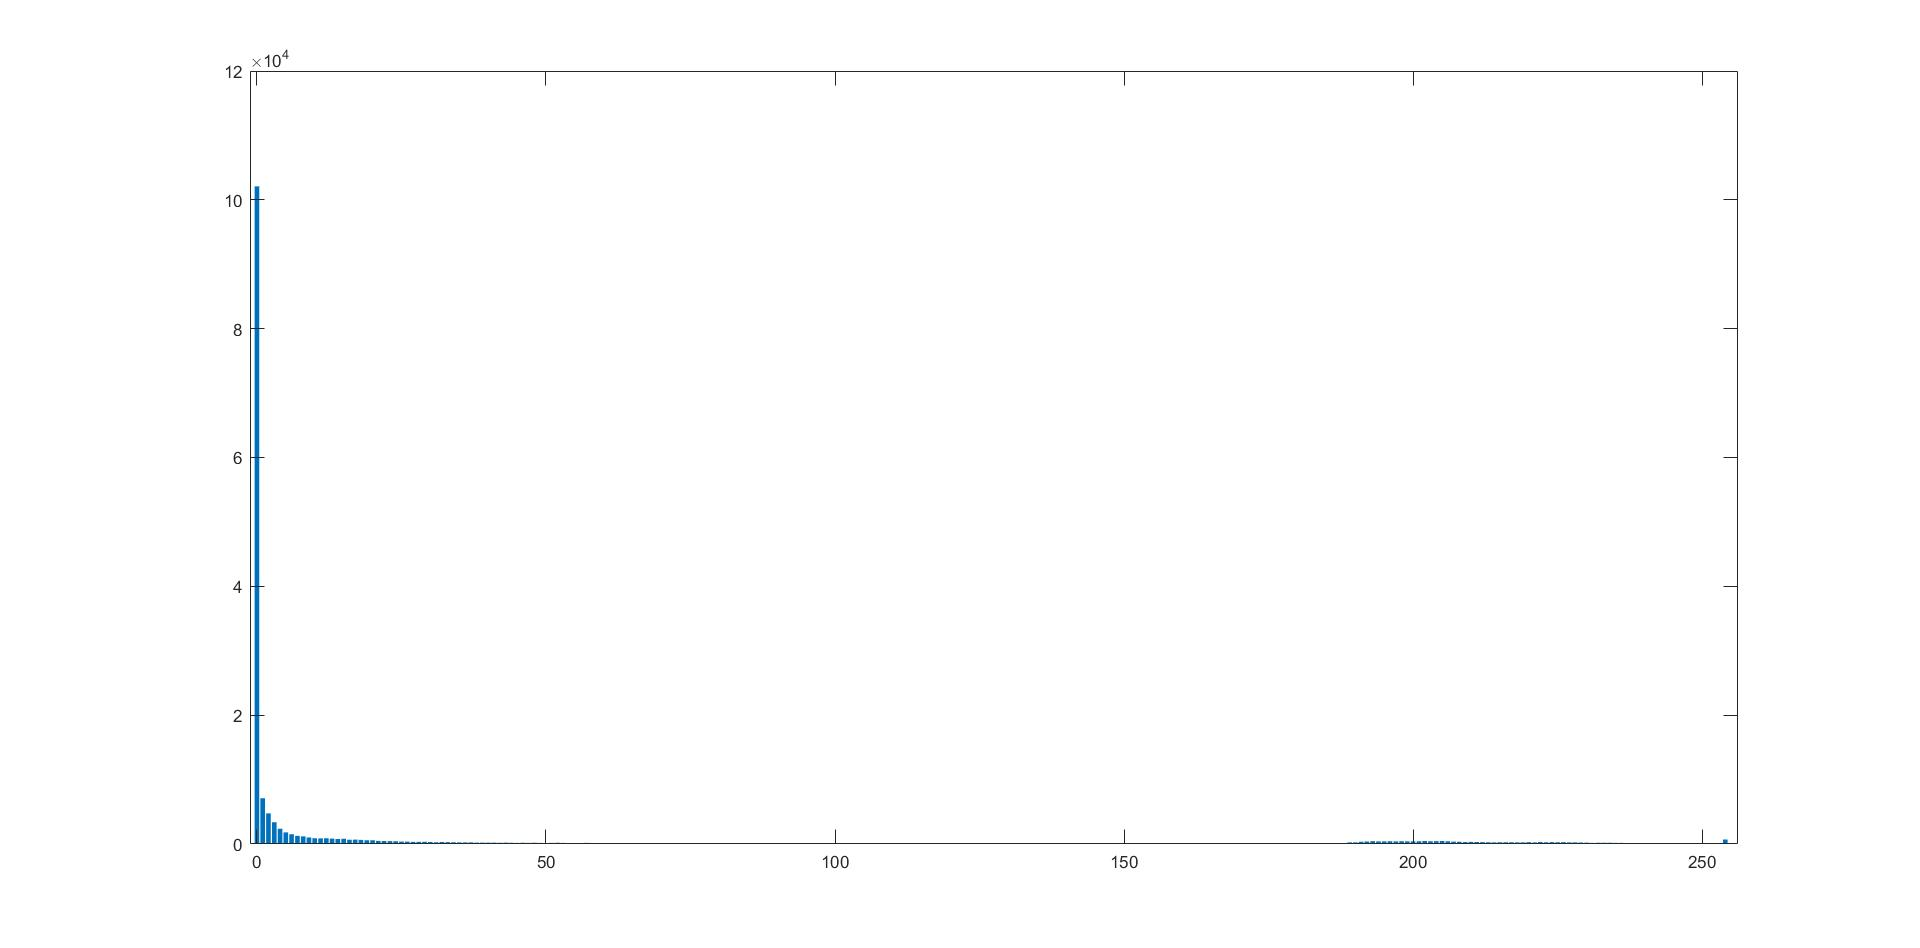
\includegraphics[width=1\textwidth]{figures/6a.jpg}
    \caption
	{
هیستوگرام تصویر \lr{Image.tif}
	}
    \label{fig:fig1}
\end{figure}


\subsection{ب}
همانطور که در هیستوگرام دیدیم، سطح روشنایی‌های صفر و نزدیک به صفر بیشتر پیکسل‌های این تصویر را تشکیل داده‌اند. اما سطح روشنایی‌های بزرگ‌تر و نزدیک به 255 هم در این تصویر وجود دارد. برای بهبود کیفیت تصویر برای سطح روشنایی‌های پایین (سطح روشنایی کمتر مساوی  \lr{k})، تابع تبدیلی می‌تواند مناسب باشد که بتواند سطوح روشنایی پایین را به محدوده وسیع‌تری نگاشت کند و از سوی دیگر قابلیت حفظ تقریبی سطوح روشنایی بالای قبلی را هم داشته باشد. بنابراین از تابع تبدیل لگاریتمی می‌توانیم استفاده کنیم. همچنین برای بهبود کیفیت تصویر برای سطح روشنایی‌های بالا (سطح روشنایی بزرگ‌تر از \lr{k})، بخش عمده‌ای از پیکسل‌ها دارای سطح روشنایی بالا هستند، ولی مناطقی شامل پیکسل‌هایی با سطح روشنایی پایین نیز در تصویر وجود دارد. این تبدیل، سطوح روشنایی بالا (نواحی روشن تصویر) را به محدوده گسترده‌تری نگاشت می‌کند. بنابراین تابع تبدیل معکوس لگاریتمی می‌تواند مناسب باشد (برای وضوح بیشتر قسمت سفید مقدار گاما را برابر با $1.2$ قرار داده‌ایم و  \lr{k} می‌تواند 127 باشد). توابع استفاده شده به ترتیب $J = 31.875\times \log (I+1)$ و $J = \frac{1}{255}I^{2}$ هستند. خروجی تصویر به شکل زیر می‌باشد.
\begin{figure}[H]
    \centering
    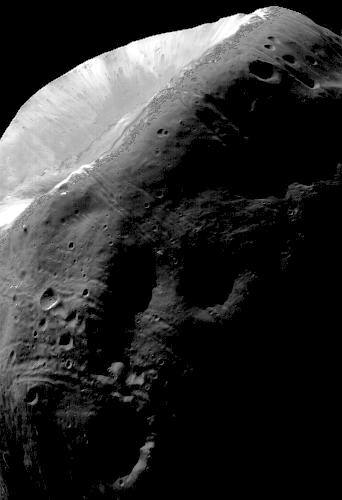
\includegraphics[width=0.5\textwidth]{figures/6b.jpg}
    \caption
	{
خروجی تابع تبدیل
	}
    \label{fig:fig1}
\end{figure}

\subsection{\lr{Code}}
\begin{latin}
\lstinputlisting{sources/p6b.m}
\end{latin}

%%%%%%%%%%%%%%%%%%%%%%%%%%%%%%%%%%%


%\begin{latin}
%\lstinputlisting{sources/p1.m}
%\end{latin}



%%%%%%%%%%%%%%%%%%%%%%%%%%%%%%%%%%%
%%%%%%%%%%%%%%%%%%%%%%%%%%%%%%%%%%%
%%%%%%%%%%%%%%%%%%%%%%%%%%%%%%%%%%%

%------------------------------------------------------------------------------------------


\section*{منابع}
\renewcommand{\section}[2]{}%
\begin{thebibliography}{99} % assumes less than 100 references
%چنانچه مرجع فارسی نیز داشته باشید باید دستور فوق را فعال کنید و مراجع فارسی خود را بعد از این دستور وارد کنید


\begin{LTRitems}

\resetlatinfont

\bibitem{b1}
\end{LTRitems}

\end{thebibliography}


\end{document}
